\section{Method}
Both the spectrums and the images will be analysed using spectrometer methods, this will open up for the opportunity to pre-process spectral and spatial data in the same way. We will then hopefully be able to compare the data more directly. The spectrometer processing method we want to use is relative reflectance ($RR$). Since this method is also being used with the spectrometer, it will be denoted $RR'$ whenever it is used for imaging. As can be seen from (\ref{eq:relative_reflectance}), relative reflectance is done by dividing the interesting values with a reference. The translation to image processing must be to divide every image pixel with a pixel value from a reference image. For comparing values with the spectrometer it is fully ok to do this division as long as the reference image is non-zero for all pixels. For that reason it is important with a well lit and preferably white background. 


One problem with this method is that images can only be visualized as three sets of integers between 0 and 255, i.e. the colors blue, green and red. Therefore we divide the division into to two cases when visualizing; reference divided by image and image divided by reference. The product will be denoted $RR'_{negative}$ for the reference divided by image case, and $RR'_{positive}$ for the image divided by reference case. The processing can be view in figure \ref{fig:image_visualization_program_flow}. Here $A$ is the image with an object and $A_0$ is the reference image. To deal with noise in the system, a noise limit is put in place before doing the division. This noise limit ensures that the difference between the image to be analysed and the reference is large enough to be assumed as a signal and not noise. This paper will later find the noise limit value with the infamous trial and error method. 

\begin{figure}[h]
    \centering
    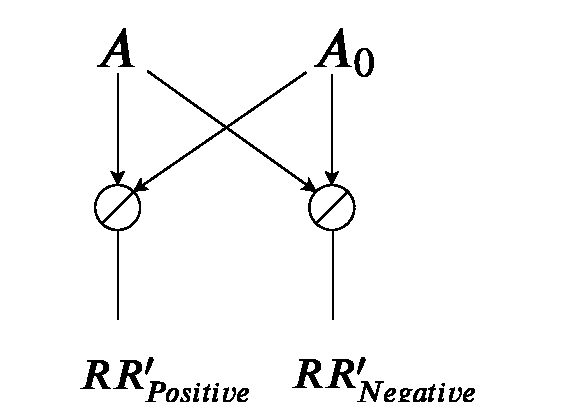
\includegraphics[width=0.5\textwidth]{figures/image_program_flow.pdf}
    \caption{Image visualization process flow}
    \label{fig:image_visualization_program_flow}
\end{figure}


\subsection{Spectrum processing}
\label{sec:spectrum_processing}

\begin{figure}[h]
    \centering
    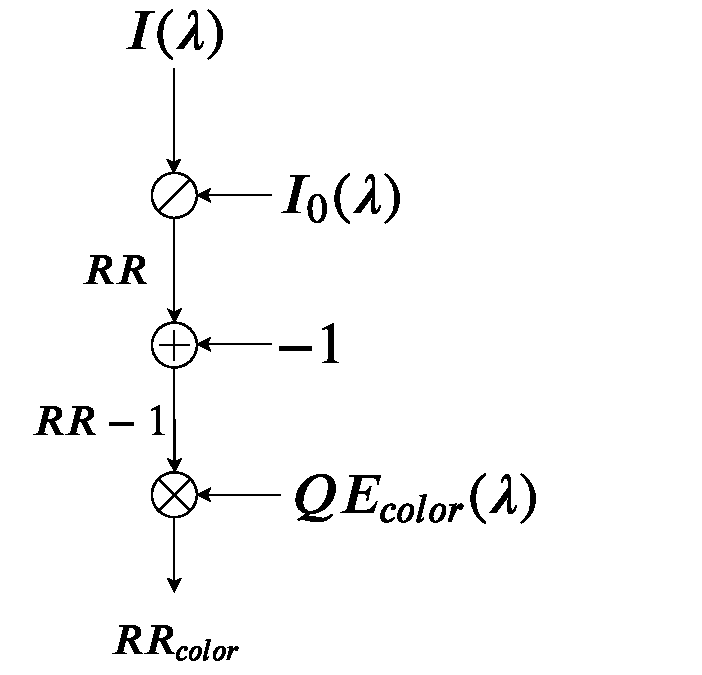
\includegraphics[width=0.5\textwidth]{figures/thesis_program_flow.pdf}
    \caption{Spectrum process flow}
    \label{fig:spectrum_process_flow}
\end{figure}

\subsection{Correlating Spectrometer to Camera}
\label{sec:method_correlating_spectrum_to_camera}
To get an idea of how well calibrated the camera is to the spectrometer and vice versa I propose the following calculation: 
Take the spatial average across the image from the camera and divide it with the spectral average of the spectrometer. 

\begin{equation}
    \label{eq:correlating_spectrum_to_camera}
    K = \frac{\mean{\vec{p}}}{\mean{RR}}
\end{equation}

This process is shown in figure \ref{fig:correlating_spectrum_and_image}.

\begin{figure}[h]
    \centering
    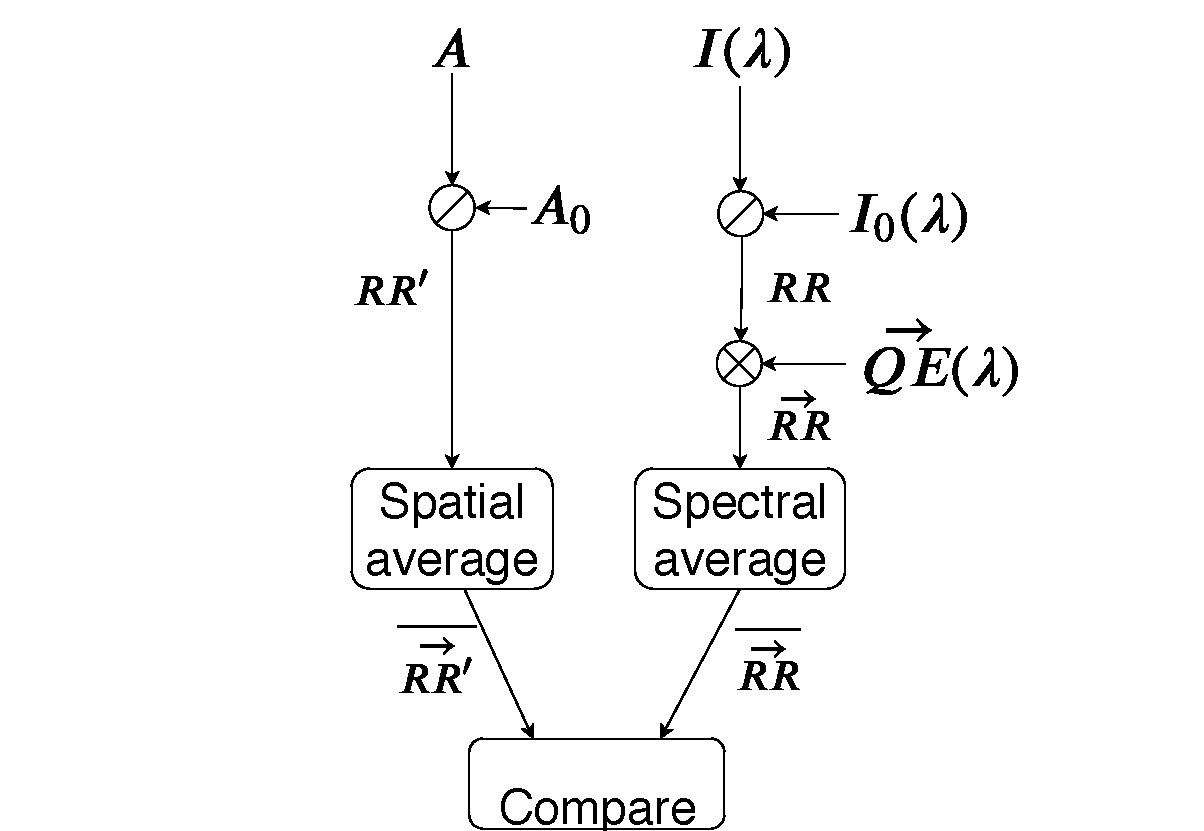
\includegraphics[width=0.75\textwidth]{figures/image_comparison_with_spectrometer.pdf}
    \caption{Correlating value between image and spectrum}
    \label{fig:correlating_spectrum_and_image}
\end{figure}


\subsection{Light}
Light is a crucial part of this project, as it is the source of input for both the camera and the spectrometer. It's also the link between the two sensors. The choosing of a sensor that can support both sensor types is therefore paramount. The camera is less selective on the spectral properties of the light source as it only requires a light source that is approximately white, i.e. have similar amounts of red, green and blue "wavelengths". It is however more selective in the spatial region as it can arise more problems for the camera if the lighting creates a lot of shadows or local problems like strong specular reflection making the pixel go into saturation. As implied the spectral properties of the light is more important for the spectrometer. For the spectrometer we want the spectrum to be as flat as possible. 

The characterization of the light source will be based on considerations from \cite{martinPracticalGuideMachine}, but also unfortunately be limited by available sources at the lab. % This paper provides a longer checklist, that can be simplified greatly under the following conditions: Stationary objects,


\section{Experimental setup}
The photos and spectrums where taken inside a lab with no external lights, and the real setup is as shown in figure \ref{fig:picture_of_setup_unlit}. %TODO: Change this figure into the side by side, lit - unlit

\begin{figure}[h]
    \centering
    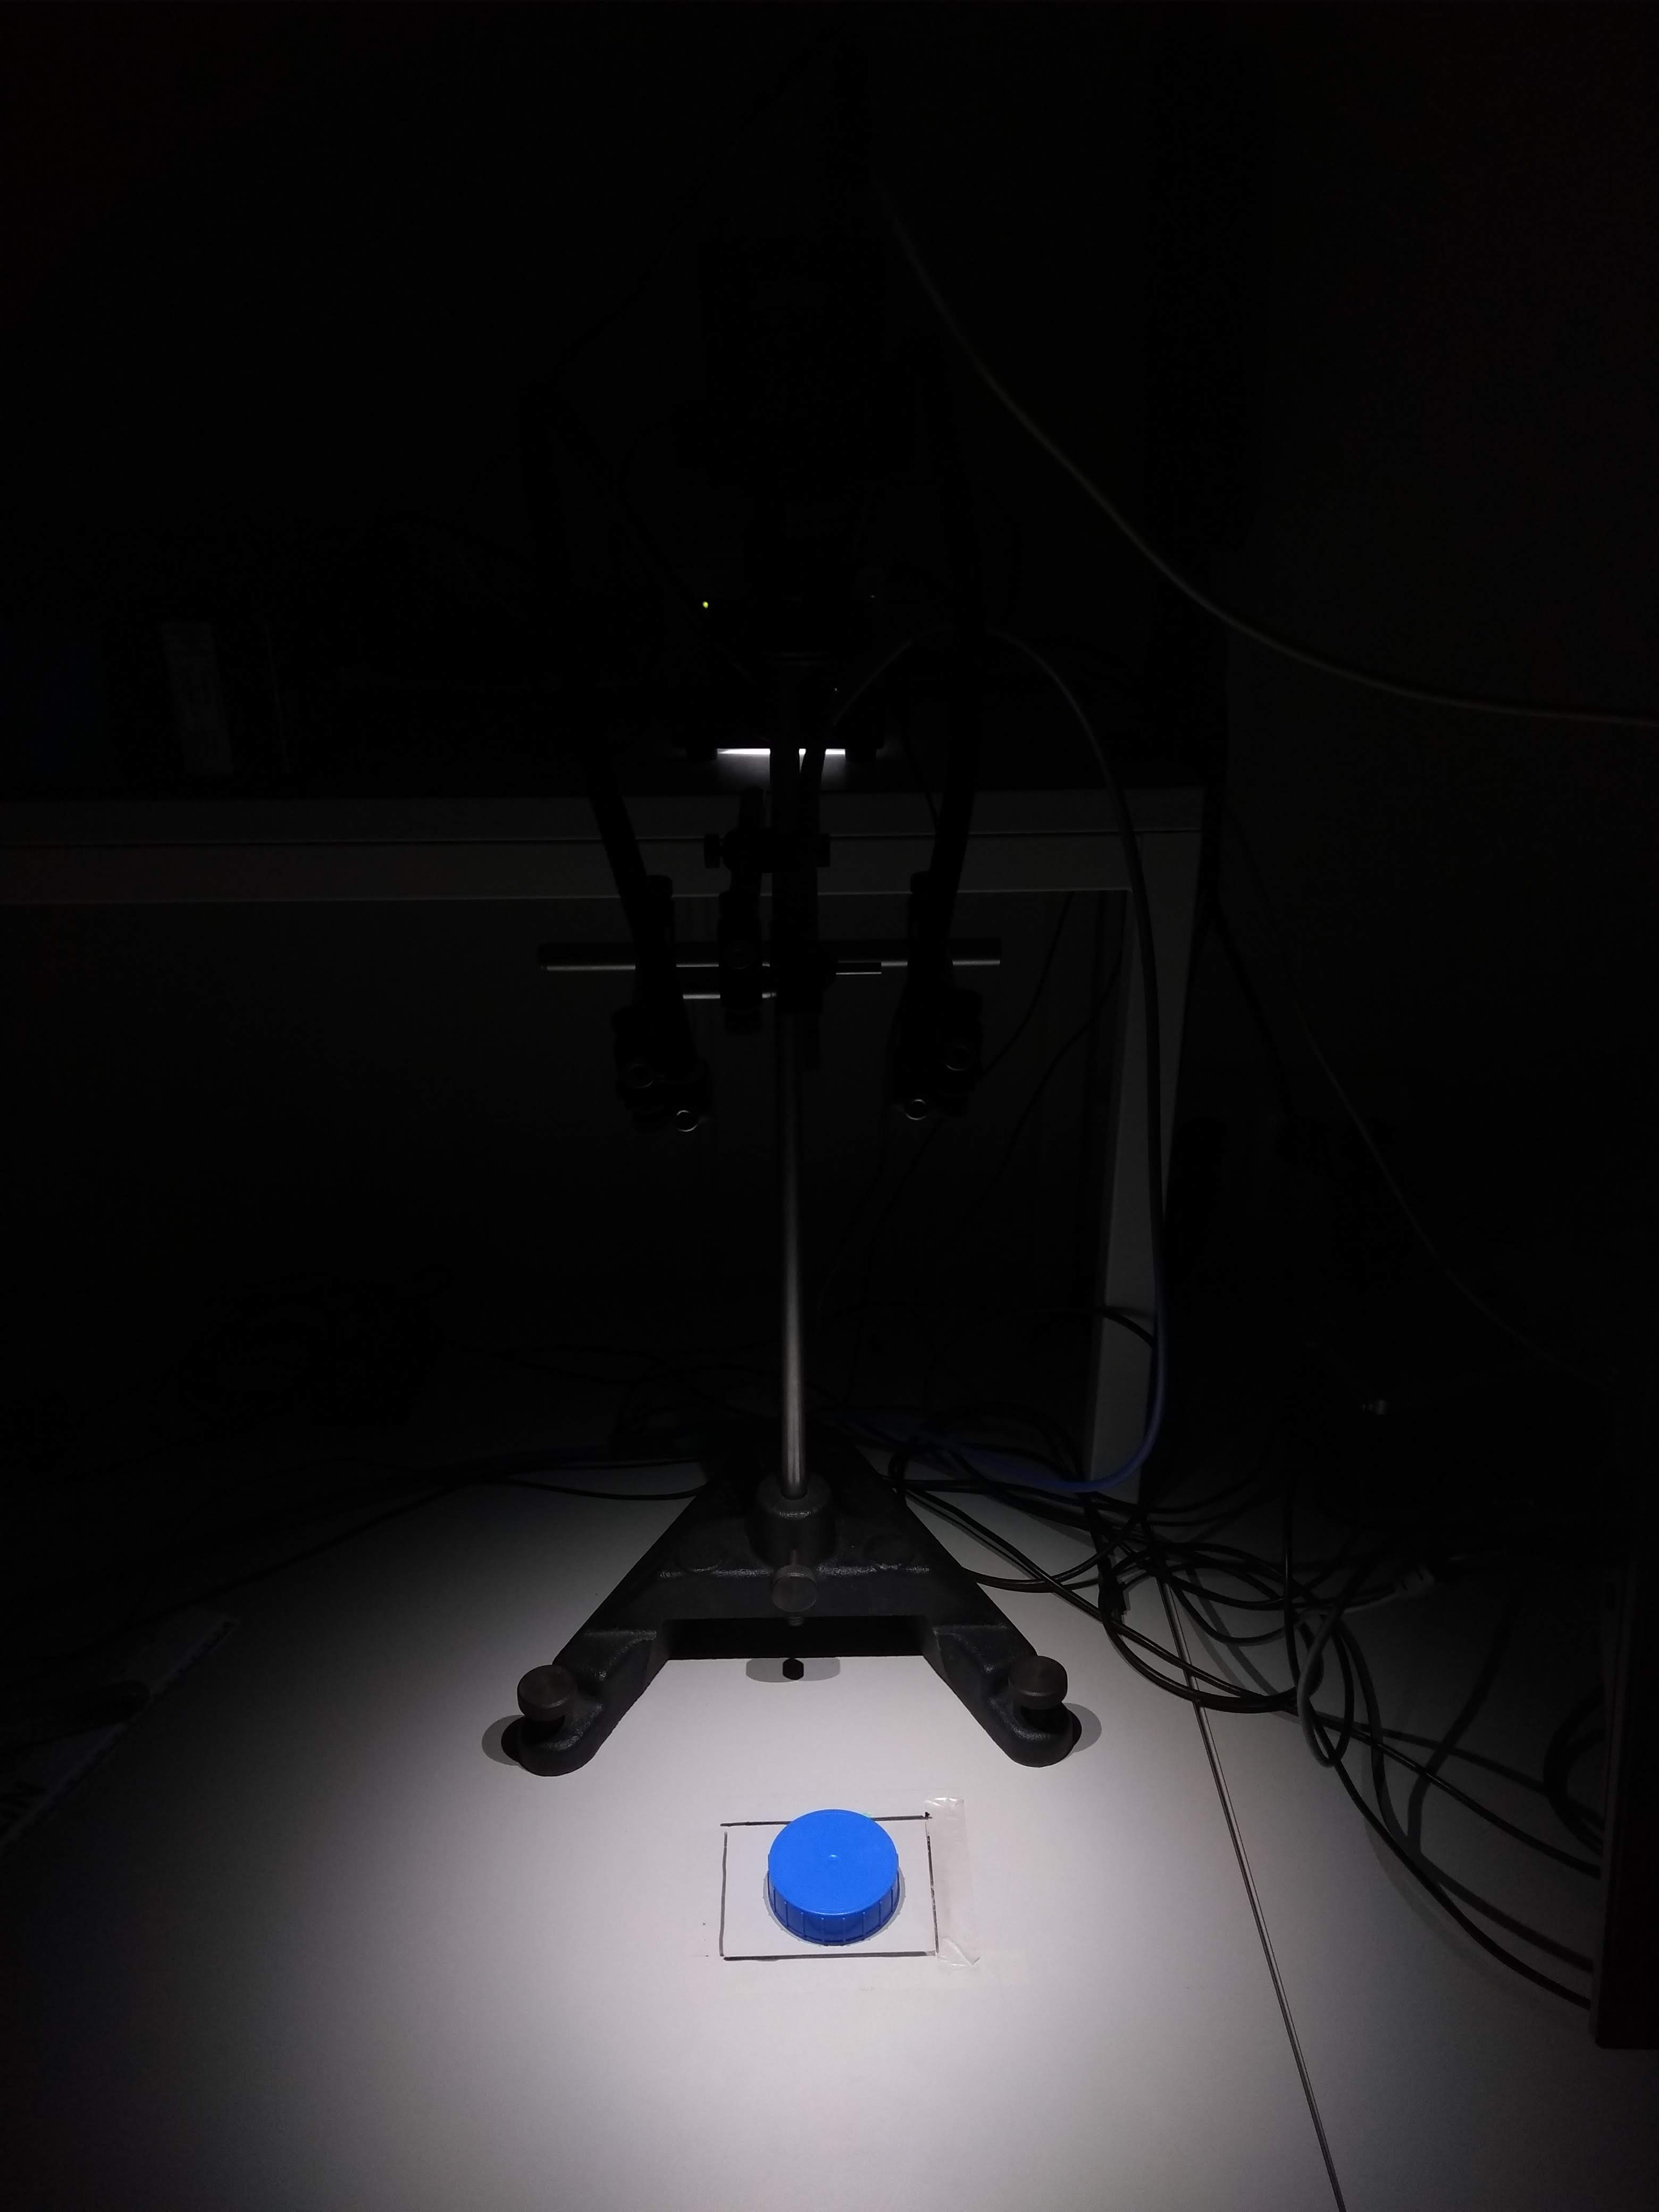
\includegraphics[width=0.3\textwidth]{figures/picture_taking_in_the_dark}
    \caption{Photo of the setup unlit}
    \label{fig:picture_of_setup_unlit}
\end{figure}

\subsection{Image processing}

To show how the processing was done, two images will be used as examples. One will be used as the reference image (figure \ref{fig:001_background}), and the other will contain an object to be analysed (figure \ref{fig:002_blue_cap}). These two images will then be sent through the process in figure \ref{fig:image_visualization_program_flow} with a noise limit of 10. 

The results from the processing are the two images in figure \ref{fig:hadamard_division_blue_cap}. They have been normalized and multiplied with 255 so that it is easy to see the changes. %TODO Are they actually histogram equalized? I don't really think so, I just normalized them and multiplied with 255.
Figure \ref{fig:002_blue_cap_positive_difference} shows what colors in what pixels have gotten more light after the blue cap was introduced. On the other hand figure \ref{fig:002_blue_cap_negative_difference} shows the colors that have gotten weaker after introducing the cap. What this means will be discussed further in section \ref{sec:blue_cap_discussion}

\begin{figure}[h]
    \begin{subfigure}{0.5\textwidth}
        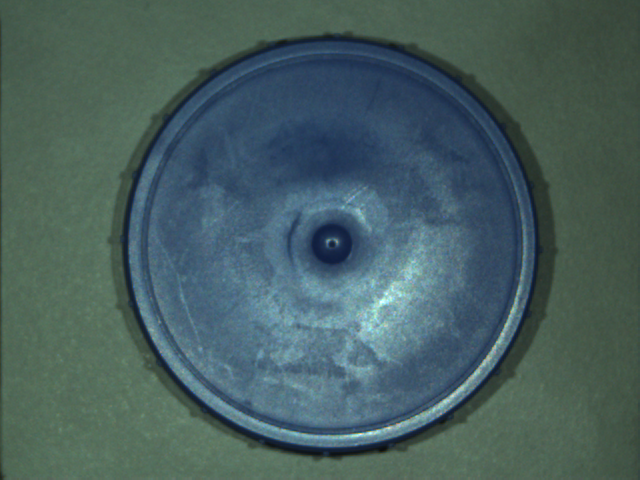
\includegraphics[width=0.9\linewidth, height=5cm]{figures/camera_pictures_png/002_blue_cap.png}
        \caption{002 Blue cap, $A$}
        \label{fig:002_blue_cap}
    \end{subfigure}%
    \begin{subfigure}{0.5\textwidth}
        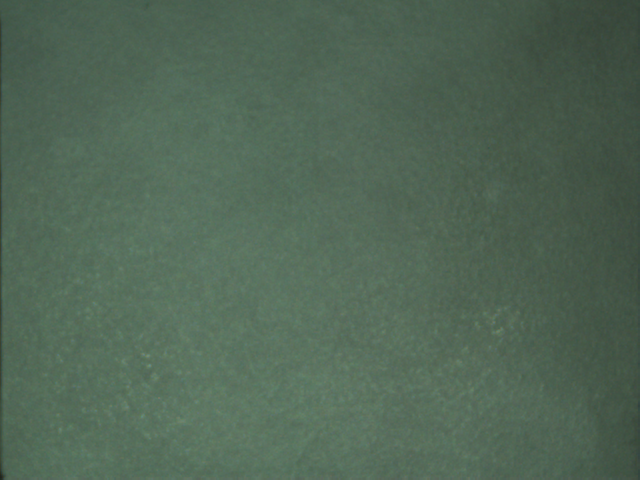
\includegraphics[width=0.9\linewidth, height=5cm]{figures/camera_pictures_png/001_background.png}
        \caption{001 Background, $A_0$}
        \label{fig:001_background}
    \end{subfigure}
    
    \caption{The original images being used in figure \ref{fig:hadamard_division_blue_cap}}
    \label{fig:blue_cap_and_background}
\end{figure}

\begin{figure}[h]
        \begin{subfigure}{0.5\textwidth}
            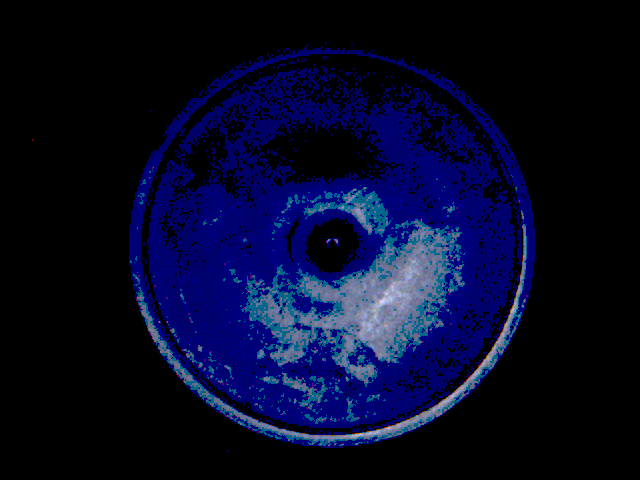
\includegraphics[width=0.9\linewidth, height=5cm]{figures/processed_camera_pictures/002_blue_cap_positive_difference.png}
            \caption{$RR'_{positive}$}
            \label{fig:002_blue_cap_positive_difference}
        \end{subfigure}%
        \begin{subfigure}{0.5\textwidth}
            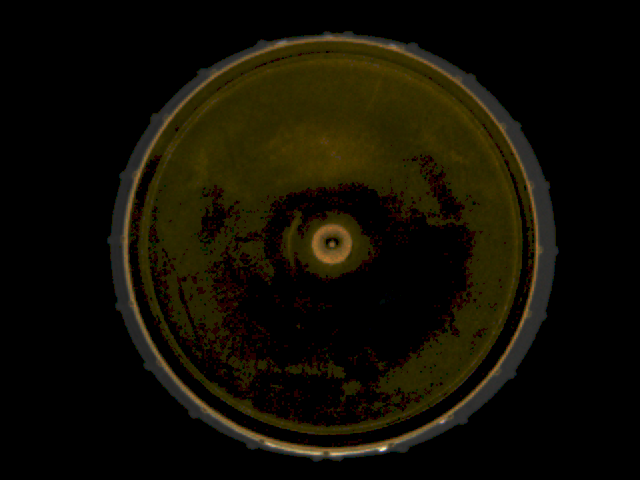
\includegraphics[width=0.9\linewidth, height=5cm]{figures/processed_camera_pictures/002_blue_cap_negative_difference.png} 
            \caption{$RR'_{negative}$}
            \label{fig:002_blue_cap_negative_difference}
    \end{subfigure}
    
    \caption{Hadamard division for the blue cap}
    \label{fig:hadamard_division_blue_cap}
\end{figure}

\subsection{Spectrum processing}

The spectrum was analysed in a similar manner, but here it was not necessary for the sake of visualization to split it into two results. It was however needed to subtract 1 from the results so that it was easy to compare the spectrums before and after multiplying with QE to each other. It also helped for comparison with the image. 
The recorded spectrums for the reference image and the blue cap is shown in figure \ref{fig:blue_cap_and_reference_spectrum}. The black line is the reference background spectrum, and the blue line is the line when the blue cap is introduced. 

\begin{figure}[h]
    \centering
    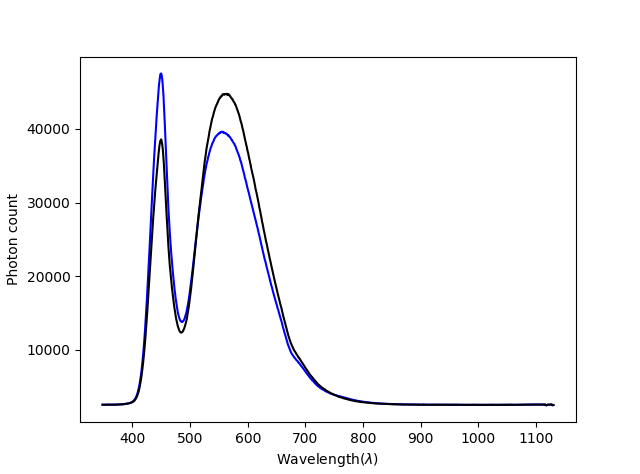
\includegraphics[width=0.75\textwidth]{Plots/blue_cap_original_spectrum_and_background.png}
    \caption{Comparison of blue cap (blue) and reference specter (black)}
    \label{fig:blue_cap_and_reference_spectrum}
\end{figure}


Figure \ref{fig:blue_cap_spectrum} shows relative reflectance minus one for the blue cap. It also includes the spectrums that the camera "sees" for each color, i.e. the wavelength parts and their respective magnitudes that is taken in by the CCD sensor. They are shown in their original colors; blue, green and red. The quantum efficiency used is shown in figure \ref{fig:quantum_efficiency_camera} in the appendix. 

\begin{figure}[h]
    \centering
    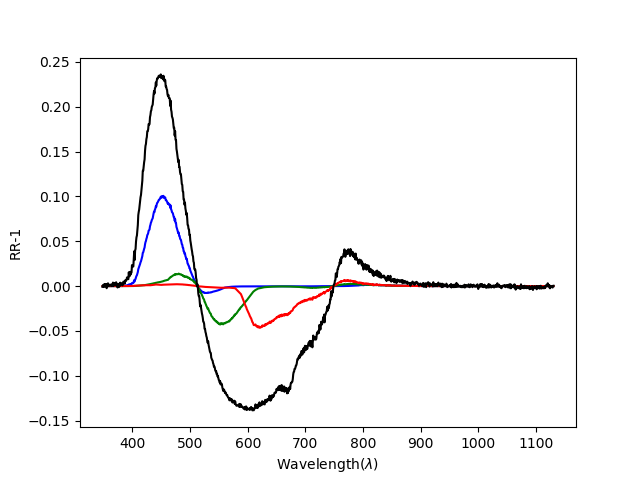
\includegraphics[width=0.75\textwidth]{Plots/blue_cap_rr_minus_one_with_qe.png}    
    \caption{Spectrum of blue cap}
    \label{fig:blue_cap_spectrum}
\end{figure}

\subsection{Spatial and spectral average}
\label{sec:spatial_and_spectral_average}

To correlate the image and the spectrum, and to get a value that describes how equal what they are seeing is, the spatial and spectral average will be used. They where introduced in section \ref{sec:spatial_average} (spatial) and section \ref{sec:spectral_average} (spectral). The idea behind using these values is that they should be linearly related to each other. %TODO1: Elaborate here while 

\subsection{Discussion of process method}

\subsection{Blue cap}
\label{sec:blue_cap_discussion}
The picture of the blue cap will be used as a basement for discussion about the image processing. 

Figure \ref{fig:002_blue_cap_positive_difference} shows what colors in what pixels have gotten more light after the blue cap was introduced. It is of no surprise that blue is the dominant here, but there are also some spots that have a strong white color. This is due to the difference between specular and diffusive reflection introduced in section \ref{sec:theory_reflection}. 

Specular reflection reflects in the same direction and will for that reason give a stronger signal than diffusive where it hits. It will however only hit if the angle between the light source, the object and the camera is just so. It is because of the strong reflection that it appears white, all three of the color sensors have reached their limit and is given out the maximum value. Specular reflection will only appear in the $RR'_{positive}$ image. 

For more diffusive parts however the light is spread in several directions and the return value to the camera is therefore weaker and it is not normal to over expose these reflections. Diffusive reflectance shows up in both $RR'_{positive}$ and $RR'_{negative}$. It is what gives us the most color to work with. 


\subsection{Spectrum of camera}

\subsection{Correlating Spectrometer to Camera}

After processing the images and spectrum as shown in figure \ref{fig:correlating_spectrum_and_image} 